\section{Processing}

\subsection{Two Step Distributed Query Processing}


MapReduce

types of files that can be processed with mapreduce

physical vs logical architecture

shuffle done with HTTP calls (moving data) - optimize shuffle with combining

block vs split vs shard

mapreduce examples-MR to sql relational algebra mapping

java API (job vs slot vs task etc - careful) good slot example in video 9.1

inputformats and outputformats

again block vs split


\subsubsection{MapReduce}

See reading assignment "MapReduce: Simplified Data Processing on Large Clusters". The following is a brief summary of that paper (enhanced with extra notes from the lecture).

\paragraph{Introduction}
\begin{itemize}
    \item \textbf{Programming model and implementation to process and generate large data sets.}
    \item \textbf{Map:} User-specified map function that processes a key/value pair and generates a set of intermediate key/value pairs. Intermediate value with the same key are grouped together.
    \item \textbf{Reduce:} User-specified reduce function that merges all intermediate values associated with the same intermediate key.
    \item Programs are automatically parallelized.
    \item Run-time system partitions input data and schedules execution across set of machines.
    \item Example: count number of occurrences of each word in a large collection of documents. Map: create (word, 1) pairs and group them together into (word, 1, 1, ..., 1) objects. Reduce: go through each object and count the ones together to create (word, n) pairs.
\end{itemize}

\paragraph{Programming Model}
\begin{itemize}
    \item \textbf{Map Type:} (k1, v1) $\longrightarrow$ list(k2, v2)
    \item \textbf{Reduce Type:} (k2, list(v2) $\longrightarrow$ list(v2)
    \item Input keys and values normally from different domain than output keys and values. Intermediate keys and values same domain as output keys and values.
\end{itemize}

\paragraph{Implementation: Execution Overview}
\begin{itemize}
    \item Partition input data into $M$ splits.
    \item Map invocations are distributed across multiple machines, processing input data in parallel.
    \item Partition intermediate key space into $R$ pieces with a partitioning function (e.g. hash(key) mod $R$). $R$ and function is user-specified.
    \item Reduce invocations are distributed across multiple machines, processing input data in parallel.
    \item Ideally, $M$ and $R$ are much larger than number of worker machines. In practice: $M$ s.t. input roughly 16 - 64MB (effective locality optimization) and $R$ a small multiple of expected number of worker machines.
    \item Avoiding stragglers: when MR operation close to end, master schedules backup executions of remaining tasks.
\end{itemize}

\begin{figure}[h]
	\centering
	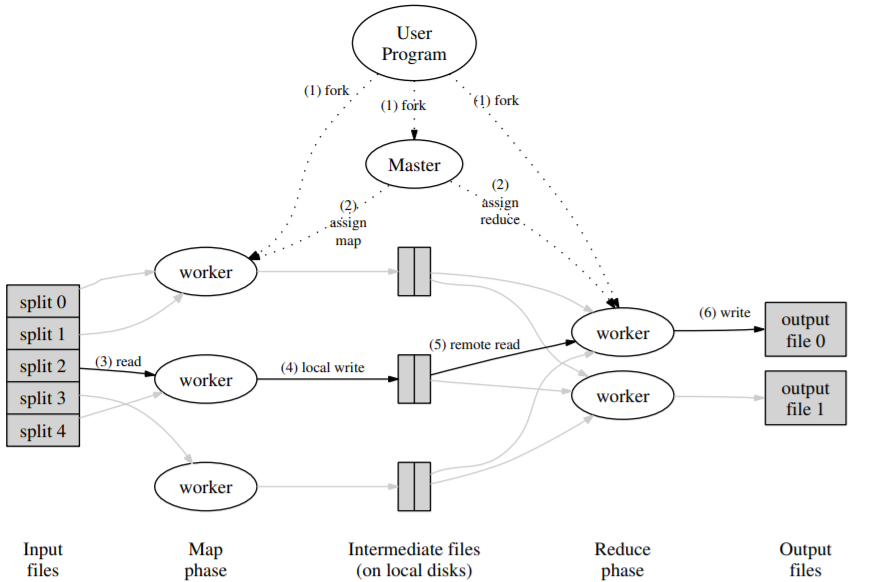
\includegraphics[scale=0.7]{images/4-MRexec.PNG}
	\caption{MR execution overview.}
	\label{fig:MR_exec}
\end{figure}

\begin{enumerate}
    \item Split input files into $M$ splits (16 - 64MB a piece). Start up copies of user program on cluster of machines (one copy = master, rest are worker programs).
    \item Master has $M$ map and $R$ reduce tasks to assign - pick idle workers and assign each one a map and a reduce task.
    \item Worker with map task: read contents of corresponding input split, parse key/value pairs, pass each pair to user-defined map function. Buffer intermediate key/value results in memory.
    \item Buffered pairs are periodically written to local disk that is partitioned to $R$ regions by partitioning function.
    \item Master notifies reduce worker about locations of intermediate key/value pairs. Worker uses remote procedure calls to read buffered data from local disks of map workers. All read - sort by intermediate keys (grouping). Use external sort if this doesn't fit in memory.
    \item Reduce worker iterates over sorted intermediate data, for each unique key, pass key and all its values to user-specified reduce function. Append output to final output file for this reduce partition.
    \item All completed - master wakes up user program and MapReduce call returns. Output is available in the $R$ output files (can be passed to another MR call s.t. user doesn't have to combine themselves).
\end{enumerate}

\paragraph{Implementation: Fault Tolerance}
Master keeps track of workers and re-schedules map tasks on worker failures (even completed map tasks since they're stored on local disk - inaccessible). Completed reduce tasks don't need re-schedule, output is stored in global file system.

Master failure is rare - MR task is simply aborted if it fails, clients retry.

\paragraph{Implementation: Locality}
Locality to conserve network bandwidth. Underlying architecture is GFS - files divided into blocks and replicated on different machines. Master tries to schedule a map task on machine with or near a replica of that task.


\paragraph{Refinements: Combiner Function}
The intermediate data is shuffled around s.t. the reduce workers can process it (fetch from map workers local disks). To optimize amount of I/O, we can use a combiner function. A map worker can combine the data when flushing it to disk (or when compacting in HBase).

The combiner function is identical to the reduce function if: key/value types are always the same for input/output of combiner and reduce function and reduce function is commutative and associative.





%TODO split != block

%TODO Hadoop / HBase MapReduce from lecture - mandatory reading zsf, slot?

%TODO JavaAPI?


\subsection{Resource Management}

\paragraph{MR Master / JobTracker Responsibilities}
\begin{itemize}
    \item Resource management
    \item Scheduling jobs
    \item Monitoring workers
    \item Job life cycle monitoring
    \item Fault tolerance
\end{itemize}

\paragraph{Issues}
\begin{itemize}
    \item Not scalable
    \item Bottleneck
    \item Jack of all trades
    \item TaskTrackers / Workers are divided into slots, each possibly taking on many map tasks (or reduce tasks) exclusively. Slots with reduce tasks are idle until slots with map tasks finish.
\end{itemize}

Issues can be fixed with using YARN. The YARN resource manager does the scheduling and application management while the many application masters do the monitoring.


\subsubsection{YARN: Yet Another Resource Negotiator}

See reading assignment "Apache Hadoop YARN: Yet Another Resource Negotiator".

\paragraph{Goal}
Separate resource management functions from the programming model (e.g. MapReduce). YARN supports fair scheduling, FIFO, capacity scheduling but not preemptive priority scheduling. %TODO is that all?

\begin{figure}[h]
	\centering
	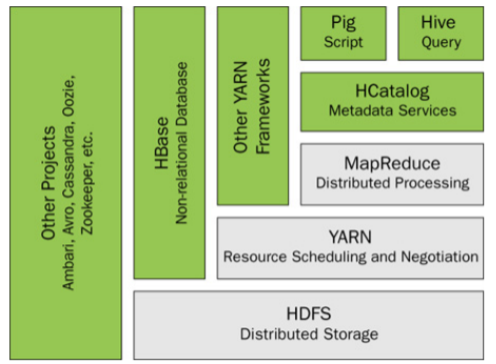
\includegraphics[scale=0.6]{images/4-yarn_hadoop.PNG}
	\caption{Hadoop components overview.}
	\label{fig:yarn_hadoop}
\end{figure}

\paragraph{Architecture}
\begin{itemize}
    \item \textbf{ResourceManager:} one per cluster, tracks resource usage and node liveness, enforces allocation invariants (fairness, capacity, locality across tenants, SLAs, not job type tho) and arbitrates contention among tenants. RM can take resources away from a running job (preemption).
    \item \textbf{ApplicationManager:} requests resources from RM, generates physical plan from received resources and coordinates execution around faults. Heartbeats exchanged with RM. Many per cluster, usually not per every node - can have multiple per node if for different applications and they are not aware of each other. AM are not privileged services in the YARN architecture.
    \item \textbf{Container:} RM schedules and dynamically allocates containers to applications. Containers are many per node and represent a logical bundle of resources (e.g. 10GB RAM and 4 cores).
    \item \textbf{NodeManager:} Running on each node (one per node) offering a container, heartbeats are exchanged with RM (resource availability, health/faults, container life cycle, liveliness, etc.). Authenticates presented tokens (container leases), manages containers dependencies, provides set of services to container, does garbage collection, etc.
    \item \textbf{Job Submission:} A job is a program (arbitrary user code / language). AM submits job and RM goes through admission control procedure. If accepted, job is scheduled and once enough resources available, job can run on spawned containers. For each container, AM gets a token that it has to present to each NM s.t. the job can start. AM can manage multiple processes (= jobs). AM itself runs in a container.
    \item \textbf{Resource Request:} AM requests to RM consist of: nr. of containers, resources per container, locality preferences and priority requests within application.
\end{itemize}

%TODO token and lease stuff - look at slides, one NM per container? logging

\subsubsection{Scheduling Strategies}

\paragraph{FIFO Scheduler}
Processes are queued and scheduled in the order that they arrive (time-based). In a shared cluster, small applications have a disadvantage.

If application 1 requests containers before application 2, subsequent container requests of a1 get served first even if a2 requested some before a1's second request.

\paragraph{Capacity Scheduler}
Different applications are guaranteed a percentage of the cluster capacity. E.g. IT department gets 60\% and Math department gets 40\% of overall capacity. Both departments then have their own scheduling algorithms, i.e. we have two separate FIFO queues. Division can be hierarchical and requests have to be renormalized to 100\% - see example in Figure \ref{fig:capsched}.

\begin{figure}[h]
	\centering
	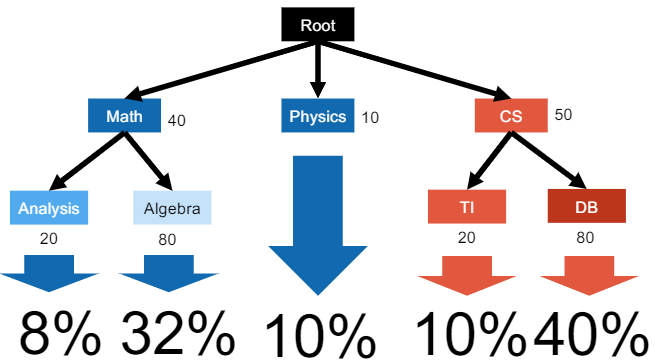
\includegraphics[scale=0.7]{images/4-capsched.PNG}
	\caption{Hierarchical queues example.}
	\label{fig:capsched}
\end{figure}

\paragraph{Cluxel}
A cluster divided into smaller chunks. For example, a cluster with 1'000GB capacity in total can be divided into 100 10GB cluxels.

\paragraph{Queue Elasticity}
If one queue is currently unused/empty, another queue can take some of its resources. We usually define capacity shares and maximum capacity allowed per class (e.g. Math can normally use 40\% of the entire cluster's capacity but if other departments are idle, it can use up to 80\% of the entire cluster's capacity). Between queues, the ones with lowest usage ratio have priority (one class = one queue).

Careful: each application of one class can still only take original share (see Figure \ref{fig:elastic}). %TODO slides differ from video on this point????

\begin{figure}[h]
	\centering
	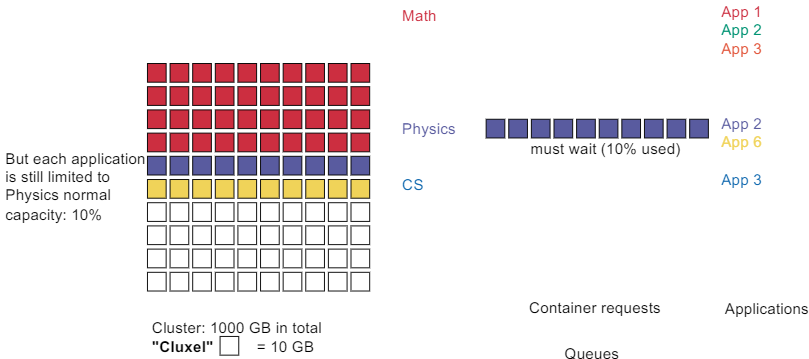
\includegraphics[scale=0.7]{images/4-elastic.PNG}
	\caption{Elastic queues example.}
	\label{fig:elastic}
\end{figure}

\paragraph{Fair Scheduling}
See next paragraphs. Different from capacity or simple FIFO queues.


\paragraph{Steady Fair Share (Soll)}
Pre-configured amount of resources reserved for each queue.

E.g.: 1'000 GB of memory, IT wants 40\%, Physics wants 10\% and CS wants 50\%. Memory is divided into: 400GB, 100GB and 500GB.

\paragraph{Current Share (Ist)}
What is actually happening in the cluster = current usage of the resources. This might deviate from the steady fair share.

E.g. IT is not using the cluster (0\%), Math is using 30\% and Physics 20\%.

\paragraph{Example: Soll vs. Ist}
Keep track of queue / class, steady fair share, current share and delta (ist - soll). We start with: Math wants 40, Physics wants 10 and CS wants 50.
\begin{enumerate}
    \item Math, Physics and CS all want to use several cluxels.
    \item Look at class with lowest delta (CS with -50) and assign 10 cluxels s.t. delta is now the same as second lowest (math -40). Update CS current to 10.
    \item Assign 40 to CS and Math each, s.t. they both match the -10 delta from Physics. Currents are now: Math 30, Physics 0 and CS 40. Cluxels in use: 70 out of 100.
    \item Physics is the only one asking, give remaining 30 to it. Deltas are now: -10 for Math, 20 for Physics and -10 for CS.
\end{enumerate}

\paragraph{Instantaneous Fair Share}
If one class is idle, re-normalize other shares to 100\%. E.g. 10\% and 50\% to 17\% and 83\%.

Replace Soll column with instantaneous fair share numbers and update deltas accordingly. Now we can see who gets more if one class stops after all was full.

If a class is still under-using while another is over-using, it can preempt the other class (harsh, usually just wait nicely) s.t. delta is 0 for all.

\paragraph{Multiple Resources}
Computing the steady fair share is easy but how to compute current share? See DRF below.

Resources can be: cores, memory, disk space, network bandwidth, etc.

\paragraph{Dominant Resource Fairness (DRF) Example}
One class uses 300GB out of 1TB memory (30\%) and 4 out of 100 cores (4\%), the other uses 10GB out of 1TB memory (1\%) and 50 out of 100 cores (50\%). For each class, take the dominant resource (mem for first, cores for second) and calculate current share by re-normalizing those, e.g. 37.5\% vs. 62.5\% usage of cluster. With this, we are back to the original algorithm. %TODO example in lecture, practice, what if dominant share changes?

Find smallest puzzle to meet steady demand and then repeat.

With this, there will be some leftover idle resources - allocate more cluxels than we actually have (since they're 2D).

%TODO YARN node manager


\subsubsection{Dominant Resource Fairness}

See reading assignment "Dominant Resource Fairness: Fair Allocation of Multiple Resource Types".

\paragraph{Goal}
In a multi-resource environment, the allocation of a user should be determined by the user's dominant share = maximum share that the user has been allocated of any resource. DRF seeks to maximize the minimum dominant share across all users.

\paragraph{Example}
\begin{itemize}
    \item Resources: 9 cores, 18GB RAM. Split them 50/50 across two users.
    \item Demands of jobs run by user A: 1 core, 4GB RAM each.
    \item Dominant resource utilization of A: 4/18 = 2/9.
    \item Demands of jobs run by user B: 3 cores, 1GB RAM each.
    \item Dominant resource utilization of B: 3/9 = 1/3.
    \item To allocate 50/50, we have A: \textbf{3} * 2/9 = 2/3 and B: \textbf{2} * 1/3 = 2/3. %TODO drawing
    \item Actual allocation: 3 * 1 (A) + 2 * 3 (B) = 9 cores and 3 * 4 (A) + 2 * 1 (B) = 14GB RAM.
\end{itemize}

%TODO practice this

\paragraph{Properties}
Properties that a resource manager should fulfill. DRF achieves all but last one in practice.
\begin{itemize}
    \item \textbf{Sharing Incentive:} Each user should be better off sharing the cluster than exclusively using her own partition of the cluster.
    \item \textbf{Strategy-Proofness:} Users should not be able to benefit from lying about their resource demands.
    \item \textbf{Envy-Freeness:} A user should not prefer the allocation of another user.
    \item \textbf{Pareto Efficiency:} It should be impossible to increase the allocation of a user without decreasing it for another (= maximize utilization).
    \item \textbf{Single Resource Fairness:} For a single resource, solution is simple max-min fairness.
    \item \textbf{Bottleneck Fairness:} If every user has the same dominant resource demands, solution for that resource is simple max-min fairness.
    \item \textbf{Population Monotonicity:} User freeing resources should not decrease any allocations in users still running.
    \item \textbf{Resource Monotonicity:} Adding more resources should not decrease any allocations.
\end{itemize}








\subsection{DAG-Based Distributed Query Processing (Spark)}
%TODO end of 9.2 clarification abt mapreduce and spark
%TODO spark intro?
%TODO RDD paper, sparkSQL paper
%TODO PySpark

\paragraph{Spark}
MapReduce is under-using YARN since YARN supports any DAG, i.e. dividing into one map and one reduce stage with a shuffle in the middle is limiting. With Spark, the data processing can follow any DAG. The dataflow does not have to be linear as in MR - we can now efficiently do iterative processing or interactive analysis of data.

Spark is best known for its ability to keep large working datasets \textbf{in memory between jobs} (instead of writing to and loading from disk in between MR stages).

Spark can run over any distributed storage system (HDFS, S3, etc.) and it needs some form of cluster management (e.g. YARN).

\paragraph{Problem of MapReduce}
It lacks the abstraction that allows it to use distributed memory. The only way to reuse data in between computations is to write and read it from disk - heavy I/O usage = bottleneck.

\paragraph{Why not simply shared RAM?}
Distributed shared memory allows reads and writes to each memory location. RDDs can only be created through coarse-grained transformations - this restricts RDDs to bulk write applications but allows for better fault tolerance. Upon failure, only lost partitions need to be recomputed (in parallel) - no need to roll back whole program.

\subsubsection{Resilient Distributed Dataset}

See reading assignment "Resilient Distributed Datasets: A Fault-Tolerant Abstraction for In-Memory Cluster Computing".

\paragraph{Introduction}
Distributed memory abstraction that lets programmers perform in-memory computations on large clusters in a fault-tolerant manner. For Spark, RDDs are one possible API (next to DataFrames/DataSets, etc.), i.e. ways to interact with Spark. DataFrames /DataSets are an abstraction of the underlying RDD abstraction.

An RDD is a collection of read-only\footnote{RDDs are resilient and immutable. Applying a transfomation to an RDD simply creates a new one - this is how we get a DAG structure. We can always read past RDDs.} structured or unstructured data items/records partitioned across the nodes of the cluster that can be operated in parallel. RDDs function as a working set for distributed programs that offers a (deliberately) restricted form of distributed shared memory.

RDDs are the nodes of the processing DAG. This is in contrast to the key/value pair files in MapReduce.

RDDs are created by starting a file in the Hadoop file system and transforming it deterministically. Upon executing an action, the transformations are actually materialized (lazy evaluation) and presented to the user (not as an RDD). Lazy evaluation allows Spark to change the DAG for better efficiency. See Figure \ref{fig:rdd}.

One can provide a partition function to efficiently partition the RDD data across nodes (exploit locality when executing Spark). %TODO true?

%TODO what exactly does an RDD look like, string? parse myself i think

\begin{figure}[h]
	\centering
	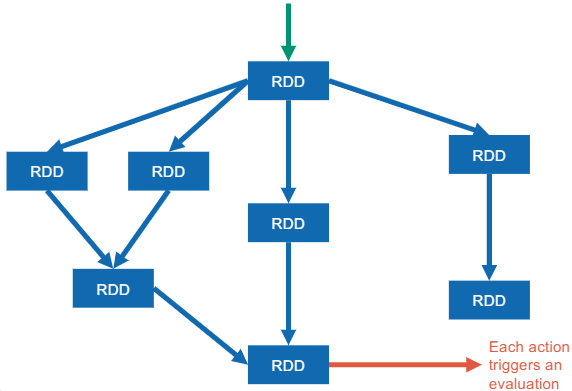
\includegraphics[scale=0.7]{images/4-rdd.PNG}
	\caption{Example Spark DAG (one creation, multiple transformations and one action).}
	\label{fig:rdd}
\end{figure}

\paragraph{RDD vs. DataFrame/DataSet Abstraction}
Since RDD is such a low-level API, a programmer actually has to think about \textbf{how} to do things, not just \textbf{what} to do (as in SQL). RDDs are best to use when we want control and we're dealing with unstructured data. But, using RDDs can make code more inefficient since Spark has less room for optimizations (Spark doesn't know what data actually is since it is unstructured and what we actually want to do with it - opaque).

\paragraph{Example Spark Execution}
\begin{itemize}
    \item \textbf{Creation:} \texttt{val rdd1 = sc.parallelize(List("Hello, World!", "Hello, there!"))}
    \item \textbf{Transform:} \texttt{val rdd2 = rdd1.flatMap(value => value.split(" "))}
    \item \textbf{Action:} \texttt{rdd2.countByValue()} 
\end{itemize}
%TODO images

\paragraph{Transformations on one RDD}
\begin{itemize}
    \item \textbf{filter:} Accept one type of value and reject another.
    \item \textbf{map:} Map each value to a new value.
    \item \textbf{flatMap:} One value can be mapped into multiple values.
    \item \textbf{distinct:} Filter out duplicate values.
    \item \textbf{sample:} Given a fraction and a random seed, sample a random amount of values. Dice at every value. %TODO fraction?
    \item etc.
\end{itemize}

\paragraph{Transformations on two RDDs}
\begin{itemize}
    \item \textbf{union:} Combine values of two RDDs into one RDD. %TODO duplicates?
    \item \textbf{intersection:} Combine all values that are the same in both RDDs into one.
    \item \textbf{subtract:} Only put values in first RDD that are not in the other in a single RDD.
    \item \textbf{cartesian product:} Clear.
\end{itemize}

\paragraph{Transformations Key/Value Pairs}
\begin{itemize}
    \item \textbf{keys:} Put all keys of input RDD into output RDD.
    \item \textbf{values:} Put all values of input RDD into output RDD.
    \item \textbf{reduceByKey:} Combine values with same key with some reduce function - makes key/value pairs with single values.
    \item \textbf{groupByKey:} Group values with same key together, values stay separated.
    \item \textbf{sortByKey:} $<=$ sort.
    \item \textbf{mapValues:} Provide function that takes values and maps into other values, same key.
    \item \textbf{join:} For each key/value pair on the left, join with fitting key on the right into key-value-value for example.
    \item \textbf{subtractByKey:} Only keep key/value pairs of left that don't have a key in the right.
\end{itemize}

\paragraph{Actions}
Output of an action is \textbf{not} an RDD!
\begin{itemize}
    \item \textbf{collect:} Output all values of result RDD.
    \item \textbf{count:} Output number of final values.
    \item \textbf{countByValue:} Each distinct value is counted, output key/value pairs.
    \item \textbf{take:} Output n first values.
    \item \textbf{top:} Output n last values.
    \item \textbf{takeSample:} Randomly output n values.
    \item \textbf{reduce:} Reduce all values into one (e.g. add up numbers). %TODO how command?
    \item \textbf{countByKey:} For each key, count same key/value pairs. %TODO value same?
    \item \textbf{lookup:} Given key, output its value.
\end{itemize}

%TODO cheat sheet of the above?

\paragraph{Persisting RDDs}
If the transformation sets for some or all actions at the bottom of the DAG overlap, don't recalculate intermediate stages for better performance. Use persisting RDDs instead = pre-calculation of subset of DAG (higher-levels). Typically one RDD. %TODO more? images?



\subsubsection{Physical Layer}

\paragraph{RDD Partition Dependencies}
\begin{itemize}
    \item \textbf{Narrow:} Each partition of the parent RDD is used by at most one partition of the child RDD. Better parallelization and locality, easier recovery.
    \item \textbf{Wide:} Multiple child partitions might depend on a partition of the parent RDD. Shuffling required.
\end{itemize}




Parallel execution: divide into tasks. Default: one task per HDFS block. Spread tasks over executors and their cores.

Sequence of parallelizable transformations: we would like it to be streamlined. Easy for narrow dependency. Divide wide dependency into stages. Job = sequence of stages.

Stage 1: all narrow, transformations stay on same machine, can run in parallel.

Shuffle: only start shuffling around until stage 1 ended.

Stage 2: again narrow, etc.

%TODO images, transf vs task vs stage vs job

Avoid wide dependency: pre-partition, e.g. key values with same key already on same machine.




\subsubsection{DataFrames}

\paragraph{Introduction}
In short: it is a distributed collection of rows with the same schema.

DataFrames (and DataSets, SQL) are a more structured and higher-level Spark API (on top of RDD abstraction\footnote{DF can also be created externally.}). DFs offer compile time syntax error detection and runtime analysis error detection (reported before a distributed job starts).

A DataFrame (i.e. table, fixed-length column store) is made up of several data items = DataSet$<$Row$>$ = attribute names, types and attribute values of one table row. Names and types are statically known (= schema).

DFs can be manipulated with relational operations or with simple RDD functions by treating a DF as a RDD of row objects. No matter what, all operations are again lazy.








%TODO more






%TODO own research?
%TODO how to program (DF vs RDD)
Can use SparkSQL with DataFrames (vs. PySpark with RDDs).
Types: %TODO
Data formats: %TODO
Catalyst optimizations
EXPLODE SQL function
pyspark - with JSON vs. dataframes = table (higher level than RDD - easier to optimize) (everything in SQL can be implemented on top of spark / mapreduce)
- fixed length col store
- dataframe data types and type mapping
- catalyst: optimize query plan (todo?)
rdbms vs. mapreduce / spark 10.4
dealing with structured types - explode function (SQL extensions) SQL dots for objects - this needs structure - heterogeinity a limit of DFs
can switch between RDD and DF with sufficient structure (see code) \url{https://www.youtube.com/watch?v=Ofk7G3GD9jk} example also here



\subsubsection{SparkSQL}

See reading assignment "Spark SQL: Relational Data Processing in Spark".

\paragraph{Introduction}
Integrate relational processing with Spark's functional programming API - despite using semi-structured data. Mix declarative vs. procedural programming models seamlessly to access and process data. SparkSQL uses the Spark DataFrame API and Catalyst (optimizer). Write it with either Java, Scala or Python.

\paragraph{Data Model}
\begin{itemize}
    \item Base types: number types, string, boolean, binary, timestamp, date
    \item Complex types: structs, arrays, maps
    \item Custom complex types
\end{itemize} %TODO more? cheat sheet? user defined functions

\paragraph{Operations}
Domain specific language, includes all common relational operations. Operators take expressions as arguments. Spark then captures structure of computation in an ASL and passed to optimizer Catalyst (not possible with RDDs!). To just use SQL, DFs can be registered as temporary tables.
%TODO inferring schemas?

\paragraph{Storage: RDD vs. DF}
DF is stored in compact columnar storage and RDD in object-based storage. Former is more compact and therefore in-memory caching is more efficient.

\paragraph{Catalyst Optimizer}
\begin{itemize}
    \item Core: library to represent trees and rules to manipulate these trees.
    \item Main data type: tree object, node object (of various types).
    \item Rules: tree-to-tree mapping, apply them using pattern matching on sub-trees, can be applied until a fixed-point is reached (no more changes possible).
    \item Used in SparkSQL to: analyze AST to resolve references and types, optimize AST, physical planning using Spark physical operators (cost-based heuristic stuff), code generation to compile parts of the query to Java bytecode.
\end{itemize}

\paragraph{Additional Features for Big Data Workloads}
\begin{itemize}
    \item Schema inference of semi-structured data, e.g. JSON document
    \item Machine Learning stuff
    \item Query federation to external DBs (instead of loading data into local processing env., execute query on external data source - reduce traffic, improve performance)
\end{itemize}

%TODO code examples (slides)

\subsection{Performance at Large Scales}

\paragraph{Bottleneck Sources}
In most systems, one of the below sources is the main source of bottleneck.
\begin{itemize}
    \item Memory
    \item CPU
    \item Disk I/O (MR and Spark are used if disk is a bottleneck)
    \item Network I/O
\end{itemize}

\paragraph{Measurements}
\begin{itemize}
    \item Latency (arrival of first piece of data), typical latencies are between ns and ms.
    \item Throughput (how fast can we transmit data), bits resp. bytes per second.
    \item Total response time = latency + transfer time.
\end{itemize}

%TODO typical numbers / rates

\begin{figure}[h]
	\centering
	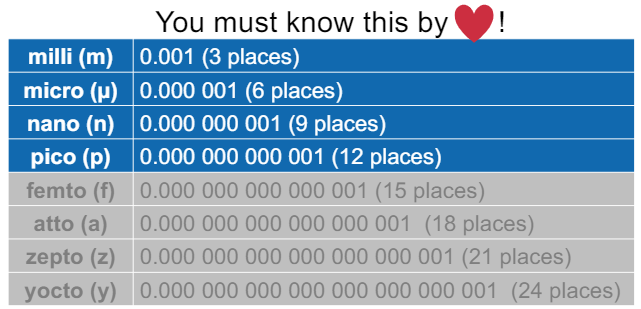
\includegraphics[scale=0.7]{images/4-units.PNG}
	\caption{Prefixes.}
	\label{fig:units}
\end{figure}

\paragraph{Speedup}
\begin{itemize}
    \item Normal: speedup = old latency / new latency.
    \item Amdahl: 1 / (1-p + p/s) where p = percent paralellizable (e.g. 0.3 for 30\%) and s = speedup on that part.
    \item Gustafson: 1 - p + s*p
    \item Amdahl assumes constant problem size (faster, same size) and Gustafson assumes constant computing power (same time, increasing size).
\end{itemize}

\paragraph{Scaling out vs. up}
Scaling up should be last resort. %TODO spark example



\subsubsection{Scalability! But at what COST?}

See reading assignment "Scalability! But at what COST?".

\paragraph{COST Metric}
Configuration that Outperforms a Single Thread.

\paragraph{Issue}
New distributed algorithms are praised for their scalability but we forget their real-world runtime performance which is sometimes worse than running a single-threaded version of the algorithm. Inefficiencies are introduced just to be scalable.



